\chapter{绪论}

\section{研究背景及意义}

\subsubsection{选题背景}

随着信息化时代的到来,公众网络产生的数据爆炸式增长。
%
企业和个人面临这海量的数据,若其独自维护这些数据,其数据可能面临着丢失、泄露的可能。
%
同时,用户也需要对数据进行计算或处理以符合自身业务需求,这也将产生巨大大的开销。
%
面对此问题,以阿里云\ucite{alicloud}、亚马逊云服务\ucite{awscloud}、腾讯云\ucite{tecentcloud}等为代表的云计算服务蓬勃发展。
%
其提供包括存储、计算、安全保护等多种数据服务。
%
用户则通过云服务提供的 API 随时随地对数据进行访问和修改,缓解了用户的数据维护成本。


然而,大多数现有的服务是中心化的,服务商对数据占有完全控制权。
%
数据可能在用户不知情中遭到泄露,或者由于服务商遭受攻击或者灾害而造成大量用户数据的损失。
%
随着区块链的发展,基于区块链的去中心化云存储(Decentralized Cloud Storage)为数据的存储和处理带来了新的可能。
%
其核心思想是充分利用网络上其他用户节点的闲置存储空间,为用户提供相对经济、海量的云存储服务。
%
现已经有较为成熟的去中心化云存储产品,例如 STORJ\ucite{storj}、Sia\ucite{Sia}、IPFS\ucite{ipfs}、Filecoin\ucite{filecoin} 等,为用户提供了不同种类的数据存储与处理服务。
%
相较于传统的 P2P 下载服务,这类产品通过以区块链发行虚拟货币的方式引入了用户激励机制,鼓励提供存储资源的用户长时间在线。
%
其去中心化的设计使用户可以自由地存储、分享数据,而不需要引入受信第三方提供服务,降低了运营商窃取用户隐私数据的风险。
%
并且,由于区块链的透明公开特性,服务商可以将也在其上维护一个公开的数据存储记录,用户可以清楚地看到数据的存储情况,一定程度上缓解了运营商的不公正收费现象。

\begin{figure}[b]
\centering
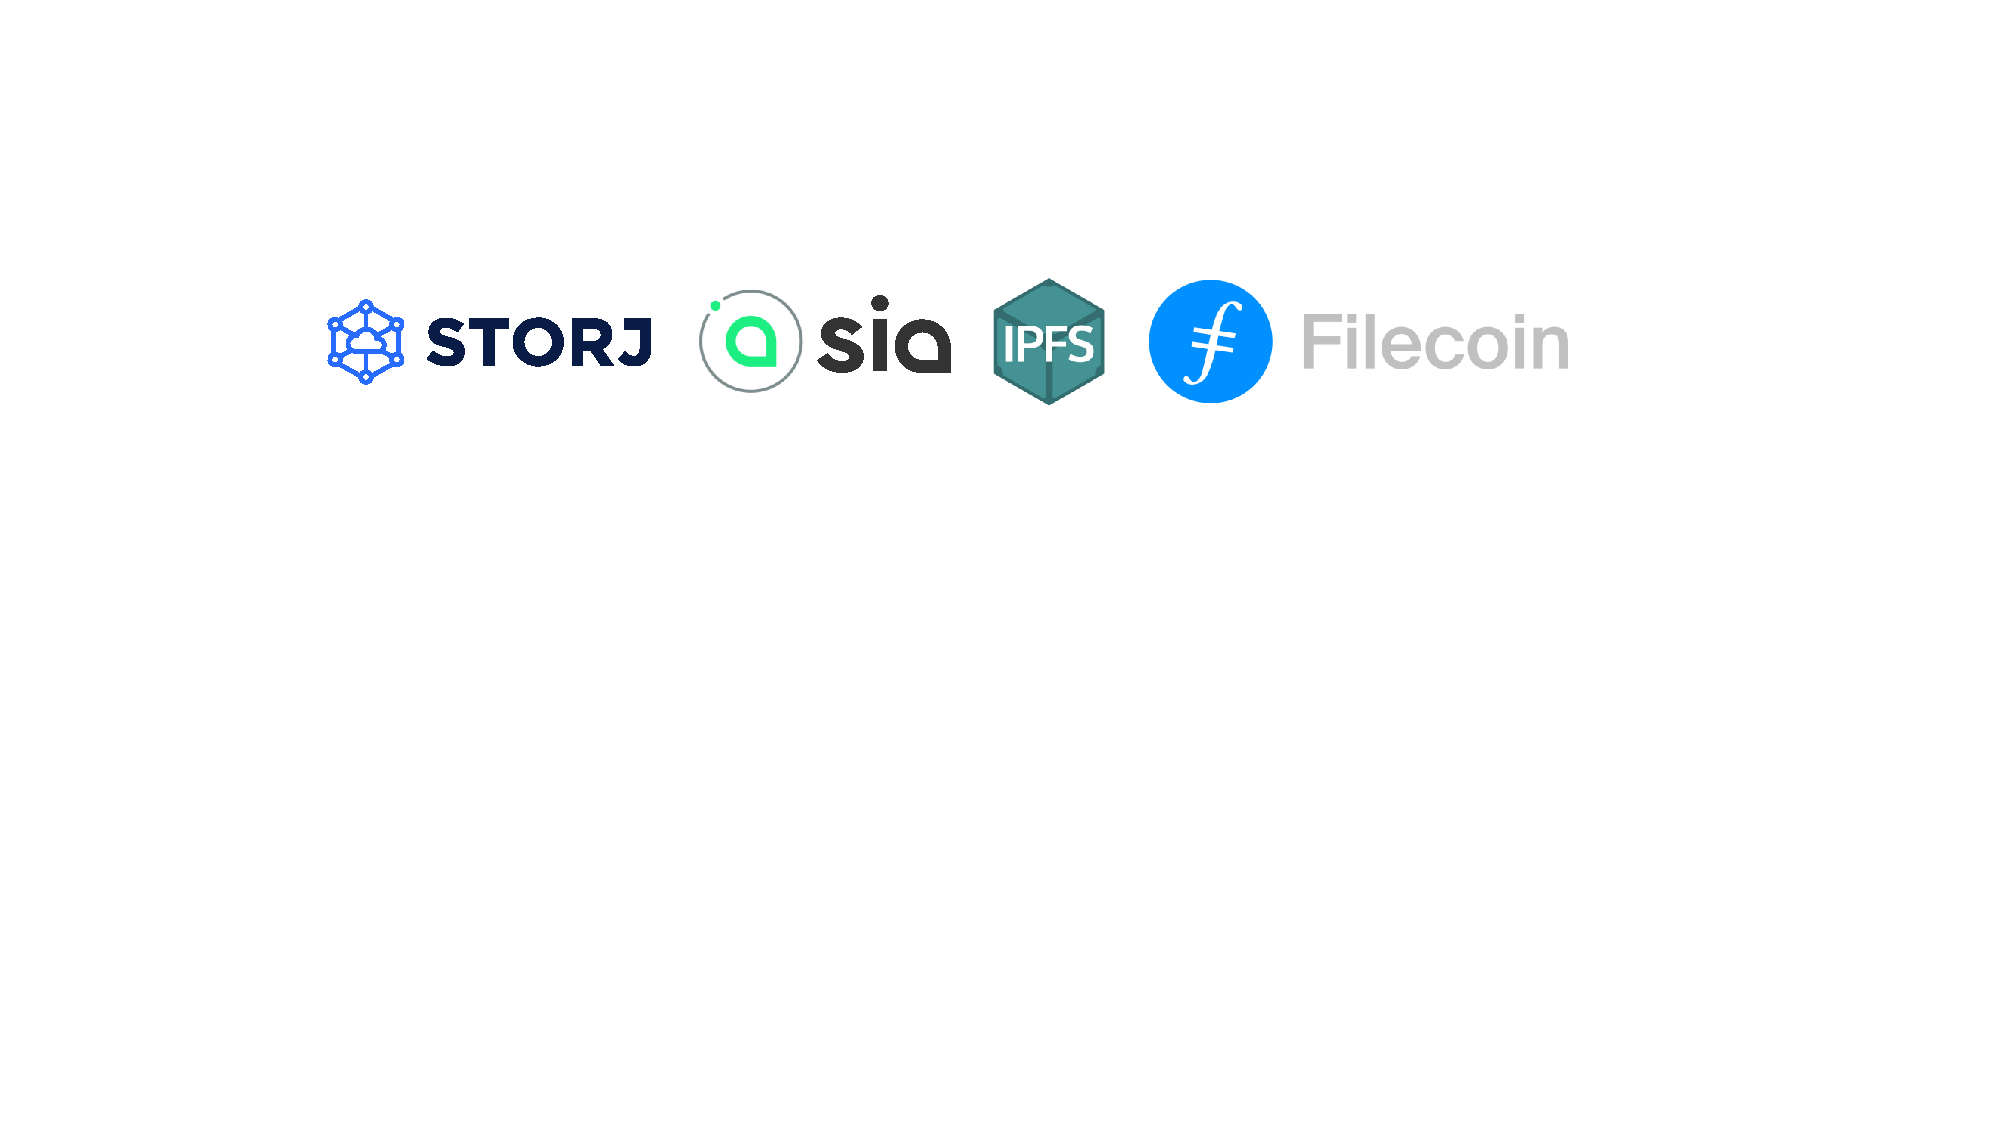
\includegraphics[width=0.9\linewidth]{fig1_clouds.pdf}
\caption{目前较为流行的去中心化云存储服务}
\label{fig-clouds}
\end{figure}

如今技术的信息化、数字化为公众带来了种种便利,许多个人、企业往往主要关注于网络产品的功能性,却忽略了“网络安全”这一重要概念。
%
在全球范围内频发的数据泄露事件,以及来自黑客的网络攻击(例如,我校邮件系统遭遇攻击等),让“网络安全”得到公众的热切关注。
%
习近平总书记在党的二十大报告中强调:“推进国家安全体系和能力现代化,坚决维护国家安全和社会稳定。”
%
因此,如何有效保障网络与信息安全,是数字时代的重要课题。
%
数据安全作为网络安全的重要组成部分,其研究具有深刻的意义。
%
在去中心化的场景下,用户的数据可能被分散存储在其他网络节点中,自然地存在数据隐私安全问题,故而隐私保护变得尤为重要。
%
因此,本选题在能够提供声称的功能的基础上,考虑各种常见的攻击以及保证数据安全,并提出解决方案。
%
本次毕业设计包含以下三个研究点:

\begin{figure}[t!]
\vskip 2ex
\centering
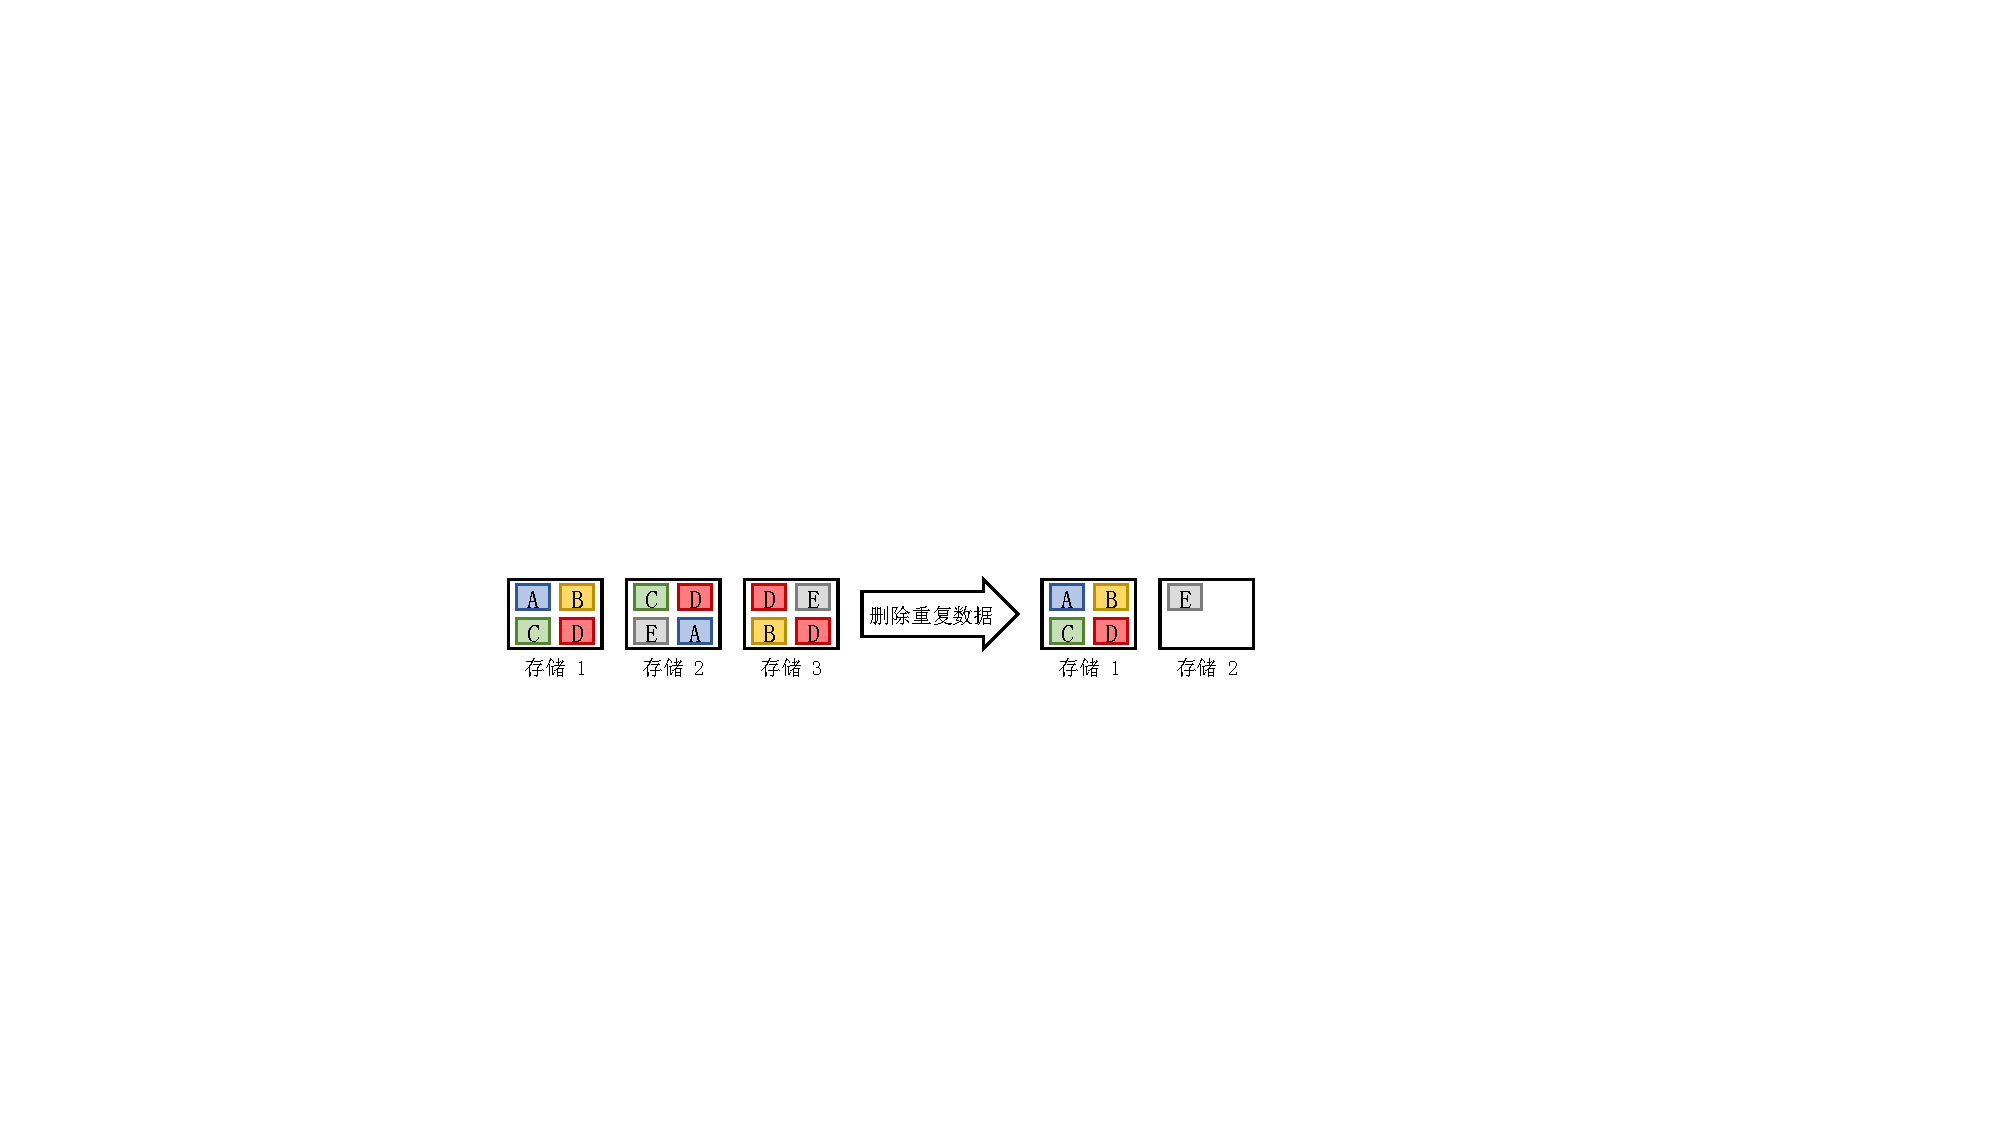
\includegraphics[width=0.9\linewidth]{fig2_deduplication.pdf}
\caption{数据去重流程示意图}
\label{fig-dedup}
\end{figure}


\begin{itemize}
\item 
\textbf{加密数据去重:}
%
用户可能将相同的数据(如公开的图片、视频等)存储到网络,进而造成大量存储的重复使用。
%
同时,许多云存储系统会通过数据冗余备份来保障数据的可用性和稳定性,会进一步加重服务器的存储浪费。
%
如图\ref{fig-dedup}所示,“去重”即为将重复的数据删除并只保存一个数据备份,可以极大的节省服务其的存储开销。
%
但这与冗余并不矛盾,因为去重可以同样减轻“无用冗余”。
%
至于数据安全,传统的加密方式(如AES对称加密)为了安全性,相同的文件将会产生不同密文,导致系统无法直接进行去重。
%
若使用确定性加密使得相同文件产生一致的密文,则可能会引入额外的网络攻击,例如,云服务器将设备离线后进行暴力破解,或不被系统发现地修改、替换用户数据等。
%
因此,有必要在考虑上述攻击的基础上提出一种加密数据去重方法。


\item
\textbf{动态用户更变:}
在用户实际使用中,数据将会根据用户需要进行删除或者修改。
%
而在去重的场景下,多个用户可能共享一个数据备份,所以系统应当妥善的处理文件所有者的变更。
%
同时考虑到数据加密机制,系统应该在不泄露额外信息的同时实现动态用户更变。
%
除此之外,由于区块链的公开透明性质,传统云存储中记录文件所有者并控制访问的方法会导致信息泄露或者潜在的恶意攻击。
%
因此,需要在保证用户隐私安全的同时在加密数据上实现动态的用户所有权更变。


\item
\textbf{地理位置验证:}
%
在去中心化网络中,节点的地理位置多样性有助于网络的稳定性和私密性\ucite{kohls2022verloc}。
%
而由于网络的虚拟性,节点的位置信息可以通过技术手段进行修改,同一用户可能通过谎称地理位置来建立更多的节点。
%
已有的地理位置验证方法通过使用公开的地标性建筑进行定位,可能会泄露部分用户隐私。
%
因此,本选题采用了最新的基于网络延迟的地理定位方案并将其整合到系统内。

\end{itemize}


\subsubsection{选题依据}

区块链以及智能合约\ucite{ethereum}的兴起,为学界以及工业界提供了可用的去中心化平台,在诸多研究领域中提供了新的研究方向。
%
智能合约通过共识机制,在全球范围内共同维护一条区块链。
%
其为合约代码的运行提供了一个全球范围内的虚拟机(例如以太坊中的EVM)。
%
合约内的代码绝对的按照既定程序运行,并且所有的合约状态均被不可篡改的记录在区块链上。
%
特别的,由于智能合约中的操作会修改大量节点的数据,因此其写入操作需要消耗实际的代币(例如以太坊中的gas)。
%
所以在设计系统时需要注意尽可能简化操作以减少代币开销。
%
同时,其安全公开的特性在数据隐私安全的场景下也会带来新的挑战,例如系统需要对上链数据设计特定的加密流程。


选题所确定的三个研究点也具备实现的依据。
%
数据去重可以在收敛加密的基础上判断相同文件密文,进而减少网络的存储开销;
%
动态用户变更通过密钥管理方法重新加密密文,使得仅有被许可的用户可以访问数据,并保证了用户隐私和数据安全;
%
地理位置的验证则通过测量节点RTT来估算目标节点的可能位置范围,可以提高系统的地理位置多样性,进而提高系统的稳定性。
%
本选题旨在结合智能合约和当今的前沿学术研究,基于区块链智能合约探索加密数据的冗余删除技术和系统实践。


\section{研究内容}

\textbf{研究目标}。
%
本次毕设目标设计一种基于区块链智能合约的去中心化加密数据冗余删除方法并实现一个示例系统。
%
该系统需要保证数据安全性和一致性,以及用户的隐私安全,允许用户删除修改文件,同时利用地理信息验证提高系统的可靠性。
%
同时系统将配备有简单的UI界面并部署在服务器上。

\subsection{基于智能合约的加密数据去重方案}

\begin{figure}[t!]
\vskip 2ex
\centering
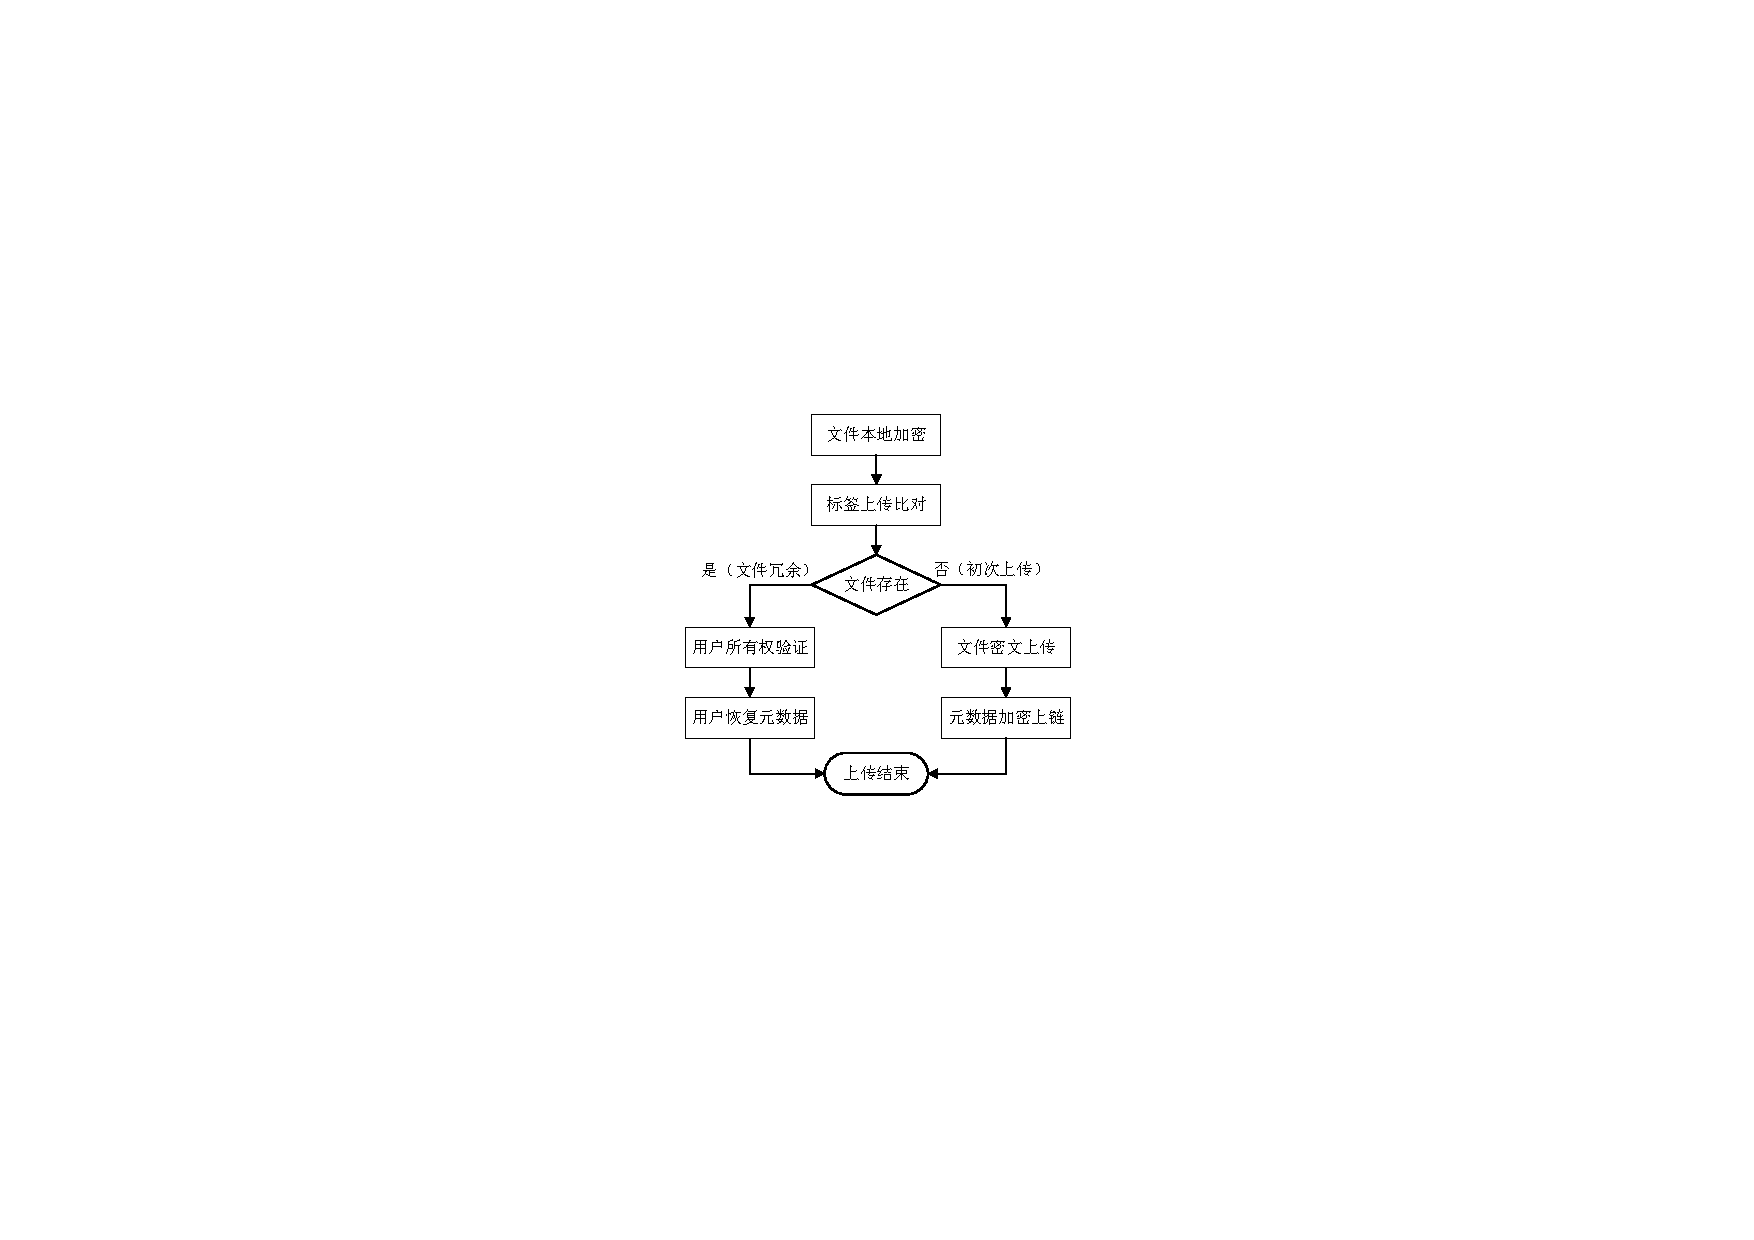
\includegraphics[width=0.5\linewidth]{figures/fig3_dedup_flow.pdf}
\caption{加密数据去重方案流程简图}
\label{fig-dedup-flow}
\end{figure}

该研究点为本选题的基础部分,后续研究点在该研究点的基础上对功能进行拓展和补充。
%
本选题旨在提出一种基于智能合约的加密数据去重方案,并要求方案保证数据安全性、一致性,考虑来自外部的恶意攻击(例如,暴力破解攻击,短消息攻击等)。
%
同时,为了减少智能合约的存储开销,方案需谨慎设计上链数据并只将必要的元数据(例如文件索引)存储在智能合约上。
%
系统的简要流程图如图\ref{fig-dedup-flow}所示。


其中,“文件本地加密”中用户使用收敛加密使得每个文件对应唯一的密文和标签。
%
然后,用户将标签上传到服务节点,由服务节点比对标签与存储在智能合约上的索引来判断文件是否存在。
%
若标签存在,则用户需要通过发送一些证明来验证其所有权,随后从区块链上读取加密的文件元数据。
%
用户解密元数据后得到密文地址,并将密钥和地址保存用于后续恢复文件。
%
若标签不存在,则文件为初次上传,用户将密文上传到去中心化云存储并得到文件地址,再将文件地址加密后作为元数据上传到智能合约的存储中。
%
具体的,加密流程还需进行谨慎设计以保证系统的数据安全性,以及抵抗外来攻击等。


\subsection{面向加密数据去重的动态用户更变方案}


\begin{figure}[t!]
\vskip 2ex
    \begin{minipage}[t]{0.48\linewidth}
        \centering
        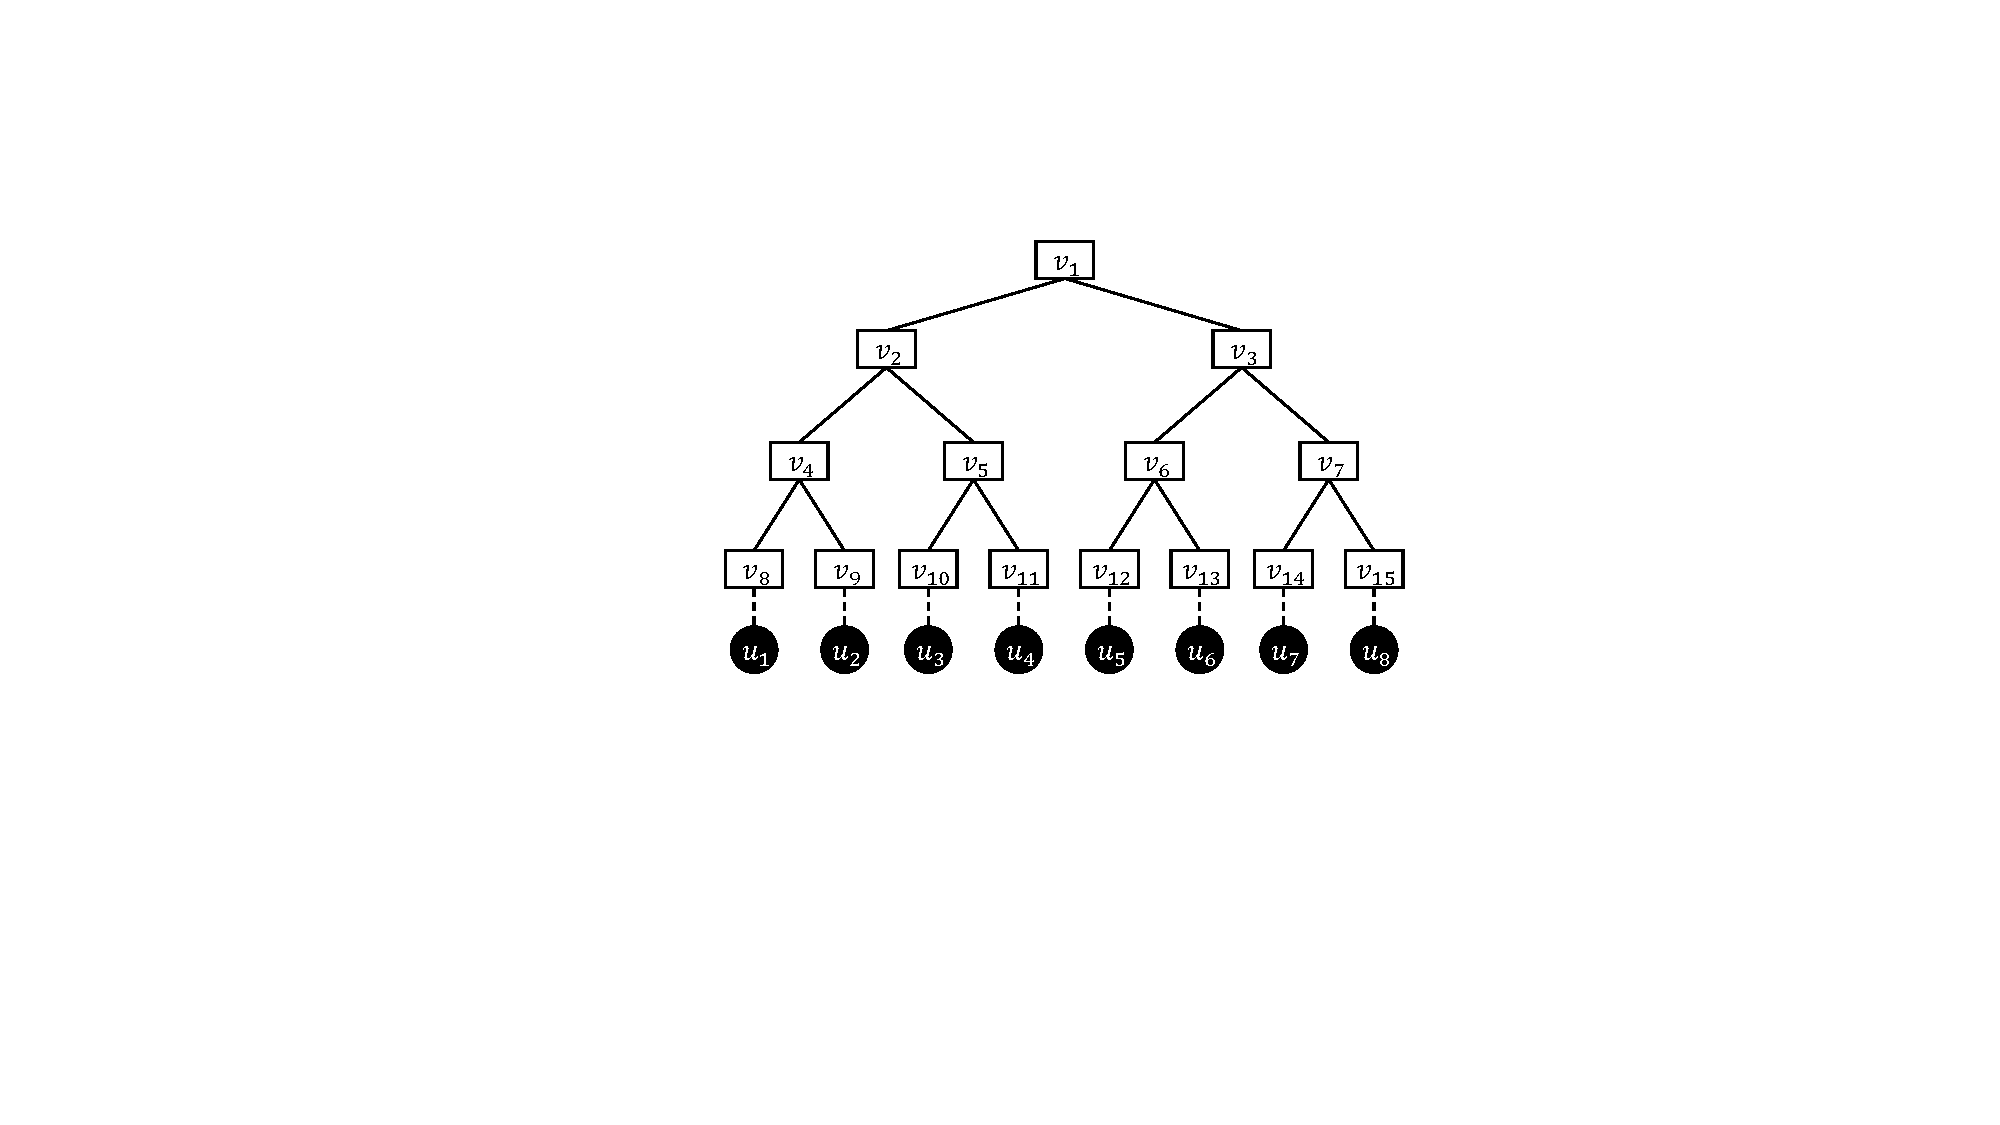
\includegraphics[width=1\linewidth]{figures/fig4_kek_tree.pdf}
        \caption{随机密钥二叉树示意图}
        \label{fig-kek-tree}
    \end{minipage}
    %
    \begin{minipage}[t]{0.48\linewidth}
        \centering
        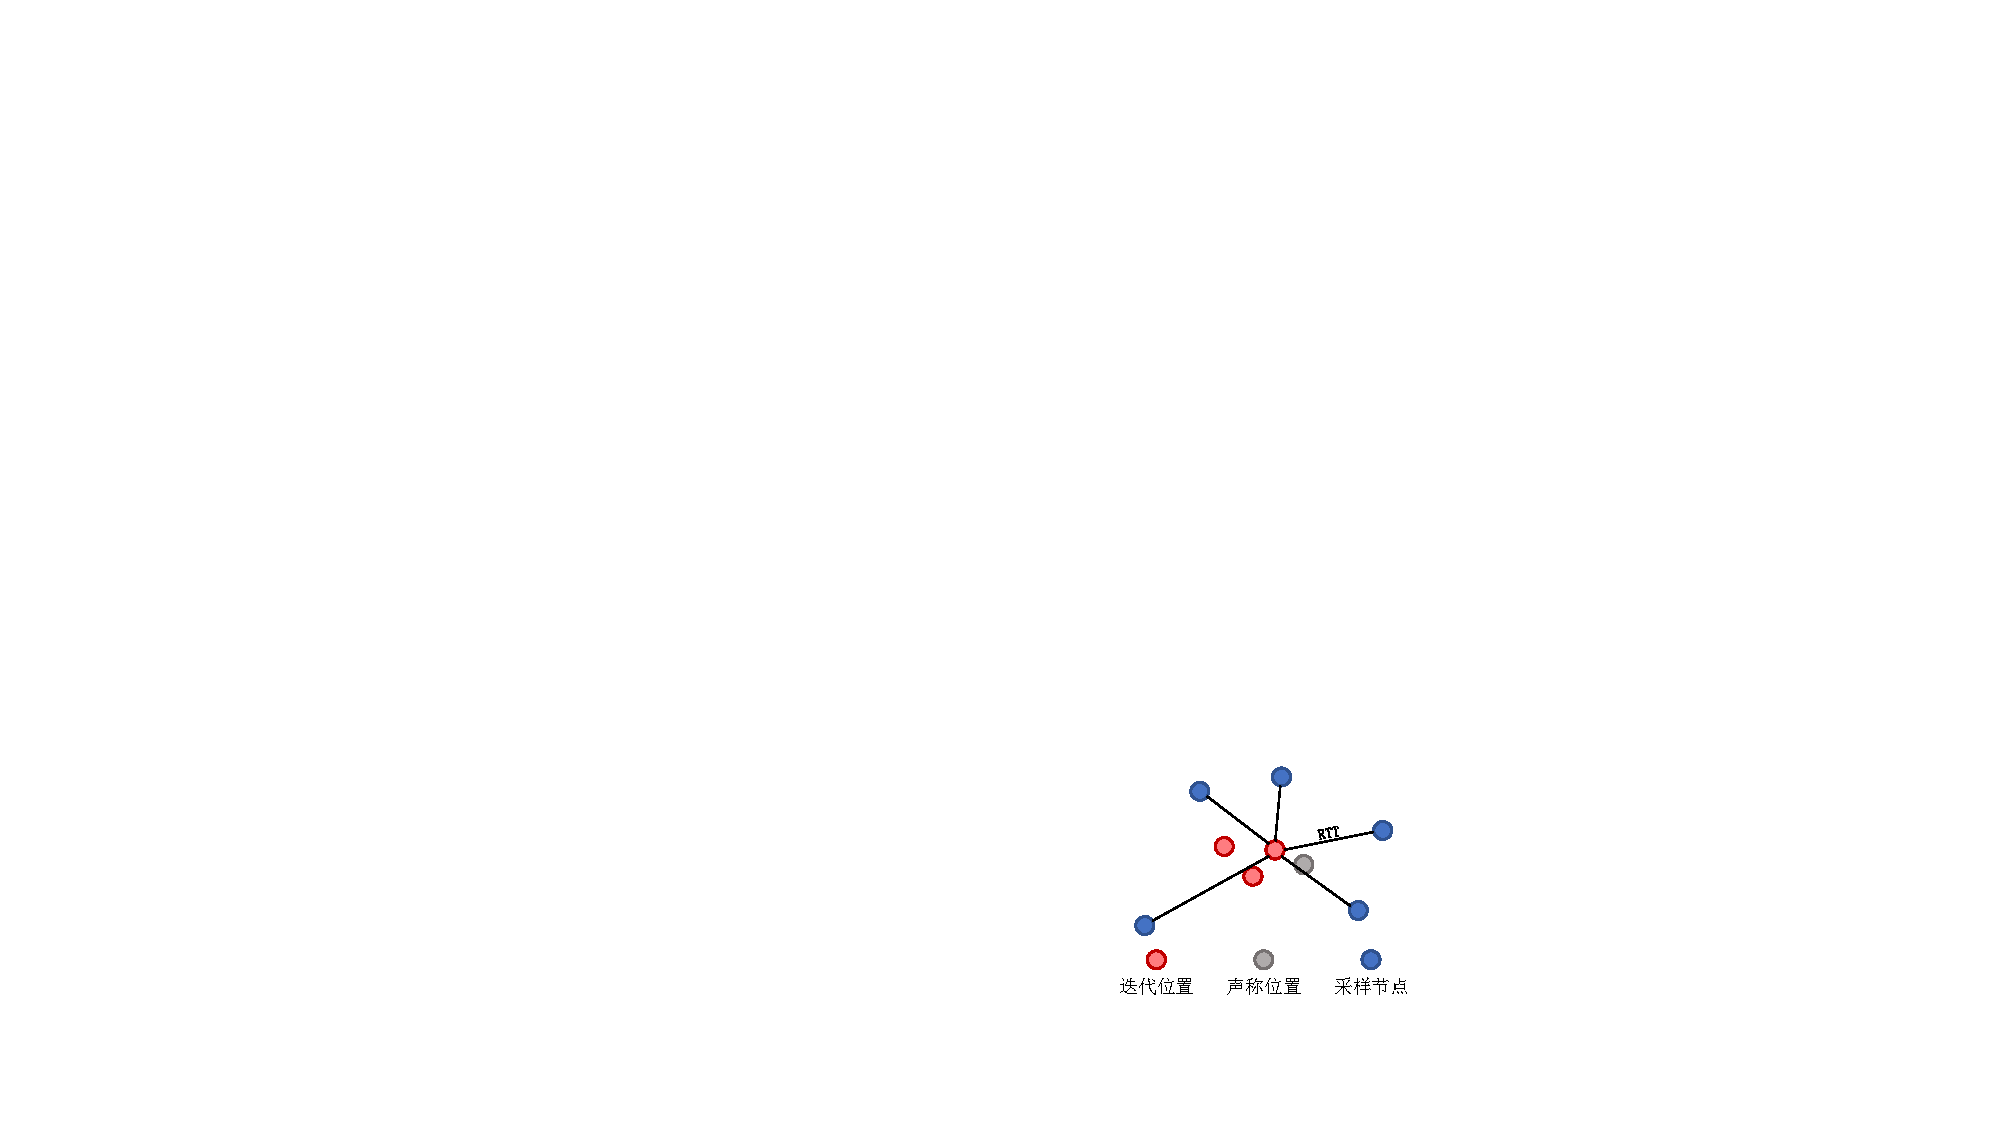
\includegraphics[width=0.8\linewidth]{figures/fig5_rtt_eval.pdf}
        \caption{RTT测距方法示意图}
        \label{fig-rtt-eval}        
    \end{minipage}
\end{figure}

本次选题采用的用户的变更通过维护系统内部随机密钥二叉树实现\ucite{ownership-management}。
%
如图\ref{fig-kek-tree}所示,每个用户$u_i$对应树的一个节点$v_j$,用户在进入系统时会收到从节点到根的路径。
%
每个文件所有者集合会对应二叉树中可以覆盖用户的最小密钥集合。
%
每当文件所有者更变时,服务节点利用随机密钥将密文再加密,再将密钥利用最小覆盖中的密钥加密随机密钥。
%
由此,只有所有者内的用户才可以解密文件加密的随机密钥,进而解密文件。
%
特别的,在去中心化加密数据去重的场景下,由于区块链的公开透明特性,系统不能像原本方法那样将二叉树直接维护在服务节点(即智能合约上)。
%
因此,本选题针对其中新出现的安全隐患进行讨论并设计抵御方案。


\subsection{基于通信延迟的地理位置验证方案}


如图\ref{fig-rtt-eval}所示,对于某个声称的节点位置,系统首先通过多个节点使用RTT进行距离测量。
%
显然,信号的传输速度不会超过光速\footnote{更具体的说,光在光纤介质中的传播速度,$2/3$光速\ucite{kohls2022verloc}。}。
%
因此根据光速可以测算目标节点到某一个测量节点的可能范围,再将多个测量节点的结果叠加,最终得到目标节点的可能分布范围。
%
系统还需要再结合实际的地图陆海分布,排除低可能性区域(如海域等),得到最终的测量结果。
%
在本选题中,由于实验条件限制,只考虑并验证了目标节点位于陕西省西安市的情况。

\medskip
此外,本选题还基于现实的智能合约实现了一个系统实例,该实例包括UI界面,以及可以接受的操作延迟,内存开销,代币开销等。


\section{\fix{国内}外研究现状}

\subsection{加密数据去重}

为了在不引入第三方服务器的前提下使得相同的文件产生一致的密文,Douceur等人提出了收敛加密(Convergent Encryption,CE)\ucite{DouceurAB2002}。
%
CE首先将文件通过哈希函数映射为一固定长度的二进制串。
%
不同的是,CE将该二进制串作为密钥,再利用确定性加密(例如,AES-CTR)加密文件得到密文,最后再将密文的哈希作为文件的标签。
%
这样,相同的文件将对应相同的密文和标签,从而可以达到去重的目的。
%
随后,Bellare等人将CE归纳为消息锁加密(Message-Locked Encryption,MLE)\ucite{MLE},并比较了多种加密方案的安全等级。
%
MLE被描述为五个多项式时间的函数,分别为密钥生成,文件加密,文件解密,标签生成和安全参数设定函数。
%
而CE可以被解释为密钥生成和标签生成函数均为哈希函数。
%
然而MLE无法抵抗可预测的数据,即由于其为确定性的,如果文件的分布集合是有限的,那么攻击者就可以通过遍历集合内部的所有文件来获取信息。
%
Bellare等人进一步提出DupLESS\ucite{dupless}。
%
DupLESS内包含一个可信的第三方密钥服务器,其内部保持一个不向任何人公开的密钥。
%
密钥服务器通过不经意伪随机函数 (Oblivious Pseudo Random Function,OPRF)对用户的密钥进行加密,并且可以保证用户和密钥服务器均不会学习到对方的信息。
%
该方法将离线暴力攻击转变为在线暴力攻击,而后者则可以通过限速策略缓解。
%
Cui等人提出了UWare\ucite{cui2018DSC},首先在文件级别、块级别提出了加密去重方法,并利用文件块的相似性推断文件相似性的方法提出了基于相似性的双级别去重方法,平衡了去重效果和计算开销。

\subsection{动态用户更变}

Hur等人\ucite{ownership-management}首次在云存储场景中提出了动态用户变更,并将前向后向安全性引入了云存储的场景。
%
其还提出了基于二叉树的密钥管理方法,系统维护一个全二叉树,每个节点包含一个随机数作为密钥,每个用户对应一个叶子节点。
%
每个用户组对应一个最小覆盖密钥组。
%
每当用户更变时,系统用随机密钥将密文再次加密,并将密钥通过密钥组加密并拼接在密文尾部。
%
每当用户删除或修改文件时,会将原本的密文重新加密,修改后的文件会重新上传。
%
保证了修改文件后的用户无法访问旧的文件(也即是,正向安全性)。
%
该工作在保证数据加密去重的基础上实现了动态用户变更,本选题考虑区块链的特性,并将该方法应用到去中心化场景中。

\subsection{地理位置验证}

传统的地理信息验证往往通过GPS等可信第三方提供位置信息。
%
\fix{在去中心化的场景下,可以通过标志性地标实现地理信息的验证。}
%
除去标志性地标外,Kohls等人提出的VerLoc\ucite{kohls2022verloc}可以利用多个节点通过通信往返时间(Round Trip Time,RTT)地理信息进行验证。
%
对于某个节点声称的地理位置,首先由多个可信节点测量RTT进行测距,再计算在不同速度条件下的可能范围,随后多次迭代得到最终的预估范围。
%
节点再通过本地数据去除底可能性地区(海域)并给出实际的可能位置。

\section{本文组织结构}

本文的组织结构如下:

本文的第二章为相关技术概述。
%
该章对系统中用到的知识技术进行了较为详细的介绍,以便读者可以更好的理解本文的工作。本文中涉及的技术主要包括区块链智能合约、密码学原语、可证明安全,以及三个研究点相关的前沿技术。



本文的第三章为加密数据去重方案设计。
%
该章首先分析了区块链的公开透明特性带了的挑战,随后介绍了去重方案的概述,包括系统构成,以及系统的安全模型和设计要求。
%
更进一步,给出了具体的方案架构,包括方案使用的数据结构和函数,详细流程和系统的安全性分析。


本文的第四章为动态用户更变方案设计。
%
该章首先介绍了在用户更变场景下的安全性需求和设计要求,随后给出了方案的具体架构设计。



本文的第五章为地理位置验证方案设计。
%
该章首先在方案概述中描述了节点距离测量的经验函数和测量的基本流程。
%
随后在方案架构设计中给出了详细的流程以及结果置信度的计算方法。



本文的第六章为系统测试与分析。
%
该章介绍了本文实现的系统原型,包括测试环境,三个方案的实现与测试结果,以及系统的UI界面展示。



本文的第七章为总结与展望。
%
该章总结了本文的主要贡献,以及对未来工作的展望。


\section{本章小结}

本章首先对论文选题的背景和研究意义进行讨论,支出了加密数据去重在去中心化场景下的挑战,然后分别介绍了本文的三个研究点。
%
随后对国内外研究现状进行了简要的介绍。

\endinput